\chapter{Generate Chart - Invalid input}
\label{chap:genChartInvInput}

\section{Input}
\label{sec:generateGanttInvalidInput}
\subsection{Project plan}
\begin{figure}[h!] 
\centering
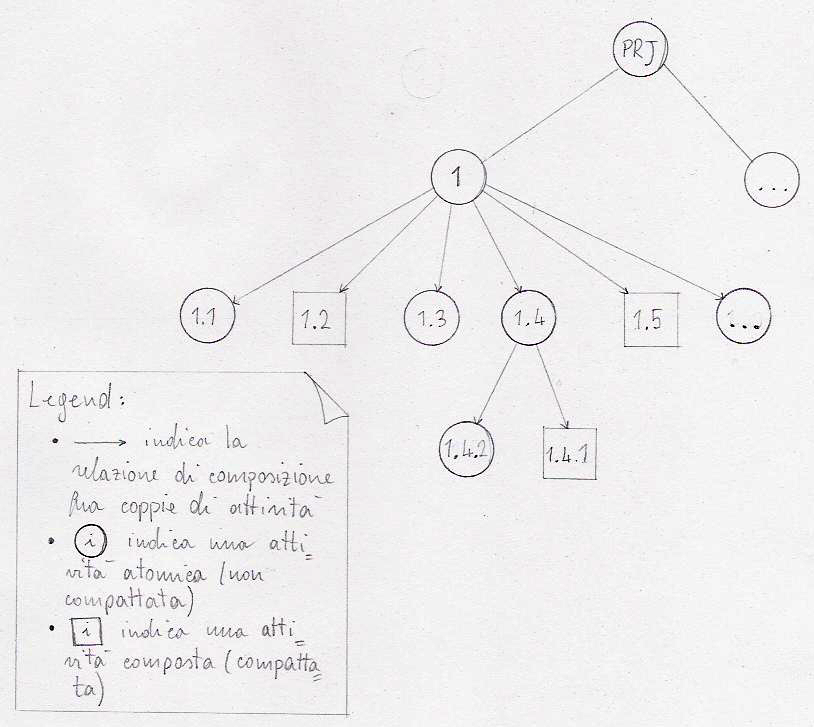
\includegraphics[width=0.6\textwidth]{case_spec/generate_Gantt/invalidInput.png}
\caption{invalid input structure}
\end{figure}

\subsection{Task definitions}
\begin{taksDef}{Task 1.4.1} \`E un task composto e la visualizzazione che si
vuole \`e di vederlo compattato; si valorizzano le propriet\`a:
\begin{itemize}
  \item $Name = ``Trasporti"$
  \item $StartDate_{planned} = 06/11/2009$
  \item $FinishDate_{planned} = 11/11/2009$
  \item $StartDate_{actual} = 07/11/2009$
  \item $FinishDate_{actual} = 12/11/2009$
\end{itemize}
\end{taksDef}

\begin{taksDef}{Task 1.4.2} \`E un task atomico; si valorizzano le propriet\`a:
\begin{itemize}
  \item $Name = ``Ordinazioni"$
  \item $StartDate_{planned} = 09/11/2009$
  \item $FinishDate_{planned} = 16/11/2009$
  \item $StartDate_{actual} = 10/11/2009$
  \item $FinishDate_{actual} = 11/11/2009$
\end{itemize}
\end{taksDef}

\begin{taksDef}{Task 1.4} \`E un task composto e si vuole visualizzare i task che lo
compongono; si valorizzano le propriet\`a:
\begin{itemize}
  \item $Name = ``Mense"$
  \item $StartDate_{planned} = 06/11/2009$
  \item $FinishDate_{planned} = 16/11/2009$
  \item $StartDate_{actual} = 07/11/2009$
  \item $FinishDate_{actual} = 12/11/2009$
\end{itemize}
\end{taksDef}

\begin{taksDef}{Task 1.1} \`E un task atomico
; si valorizzano le propriet\`a:
\begin{itemize}
  \item $Name = ``Allocazione"$
  \item $StartDate_{planned} = 02/11/2009$
  \item $FinishDate_{planned} = 06/11/2009$
  \item $StartDate_{actual} = 30/10/2009$
  \item $FinishDate_{actual} = 04/11/2009$
\end{itemize}
\end{taksDef}

\begin{taksDef}{Task 1.2} \`E un task composto; si valorizzano le propriet\`a:
\begin{itemize}
  \item $Name = ``Gestione\quad cibo"$
  \item $StartDate_{planned} = 04/11/2009$
  \item $FinishDate_{planned} = 10/11/2009$
  \item $StartDate_{actual} = 13/11/2009$
  \item $FinishDate_{actual} = 17/11/2009$
\end{itemize}
\end{taksDef}

\begin{taksDef}{Task 1.3} \`E un task atomico; si valorizzano le propriet\`a:
\begin{itemize}
  \item $Name = ``Gestione\quad Fornitori"$
  \item $StartDate_{planned} = 03/11/2009$
  \item $FinishDate_{planned} = 10/11/2009$
  \item $StartDate_{actual} = 13/11/2009$
  \item $FinishDate_{actual} = 17/11/2009$
\end{itemize}
\end{taksDef}

\begin{taksDef}{Task 1.5} \`E un task composto; si valorizzano le
propriet\`a:
\begin{itemize}
  \item $Name = ``Fatturazione"$
  \item $StartDate_{planned} = 18/11/2009$
  \item $FinishDate_{planned} = 21/11/2009$
  \item $StartDate_{actual} = 15/11/2009$
\end{itemize}
\end{taksDef}

\begin{taksDef}{Task 1} \`E un task composto; si valorizzano le propriet\`a:
\begin{itemize}
  \item $Name = ``Progetto\quad pasti"$
  \item $StartDate_{planned} = 02/11/2009$
  \item $FinishDate_{planned} = 21/11/2009$
  \item $StartDate_{actual} = 30/10/2009$
\end{itemize}
\end{taksDef}

\subsection{Task dependencies}
Possiamo creare la relazione $\sqsubset$ \emph{FinishToStart} che associa due
task in questo modo:
\begin{displaymath}
\sqsubset = \lbrace (a,b) : b_{startDate} >= a_{startDate}, \forall a,b \in
DependencyTask
\rbrace
\end{displaymath}
con \emph{DependencyTask} l'insieme di tutti i task creati definendo la
relazione di dipendenza attraverso la relativa pagina di editing disponibile in
PMango. 

Possiamo quindi applicare la definizione di $\sqsubset$ al nostro input:
\begin{displaymath}
\sqsubset = \lbrace (1.2, 1.1), (1.4.2, 1.3), (1.4, 1.5), (1.5, 1.4.2)
\rbrace
\end{displaymath}

\section{Environment}
Si vuole generare l'output con l'istanza di input sepecificata nella sezione
\ref{sec:generateGanttInvalidInput}. Come oggetti appartenti al contesto di
generazione, fissiamo queste \emph{UserOption}:
\begin{description}
  \item[TimeRangeUserOption] valorizza
  \begin{itemize}
  \item $FromStartRange = 26/10/2009$
  \item $ToEndRange = 06/12/2009$
  \end{itemize} 
  \item[TimeGrainUserOption] $= ``DailyGrain''$
  \item[TaskName] = $checked$
  \item[WBSUserSpecificationUserLevel] = $checked$
  \item[ShowDependencies] = $checked$
\end{description}

\section{Output}
\begin{sidewaysfigure}[h!] 
\centering
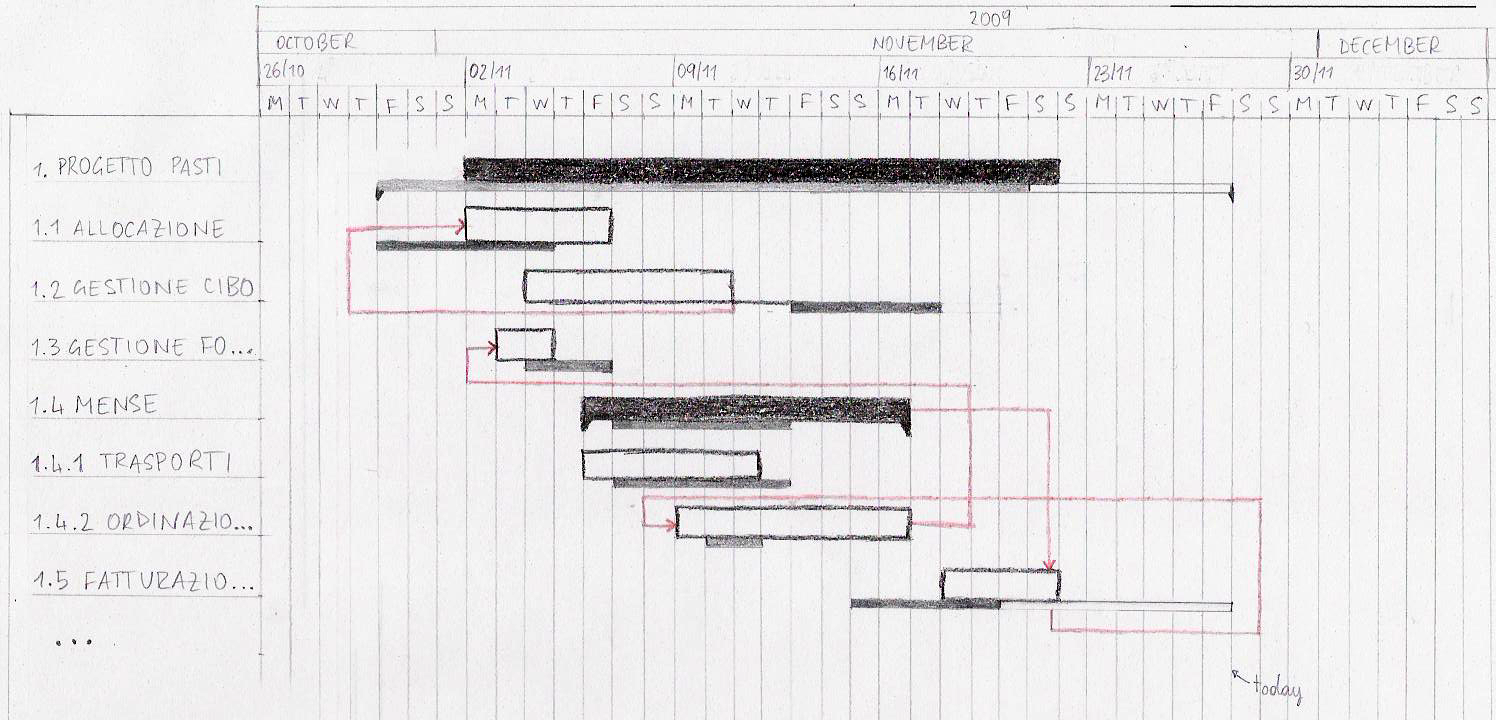
\includegraphics[width=1\textwidth]{case_spec/generate_Gantt/invalidOutput.png}
\caption{output for the invalid input structure}
\label{fig:generateGanttInvalidOutputMockup}
\end{sidewaysfigure}
See figure \ref{fig:generateGanttInvalidOutputMockup}.

\section{Pass/fail criteria}
See the figure \ref{table:passfailCriteriaGanttGeneration}.
\begin{table}[h!]
  \begin{center}
    \begin{tabular}{| l | p{100mm} |}
    \hline
    \textbf{risultato} & \textbf{criteri} \\
	\hline    
	success & 
    \begin{itemize}
  \item l'output dell'implementazione \`e sovrapponibile al modello a meno 
di una tolleranza pari a circa \textbf{1mm}
\item I punti di stacco dei segmenti
delle dipendenze possono disposti in maniera diversa da quelli esposti nel test
\item I font possono essere di una famiglia e dimensione diversa in base anche alle
UserOption scelte dall'utente.
\item Le linee verticali rappresentanti un elemento appartenente alla
\emph{TimeGrain} possono essere rappresentate (oppure non comparire affatto) in modo diverso.
\item Tutte quelle linee che sono errori di imprecisione nella stesura del mockup non
sono da considerarsi valide per il confronto (si lascia al buon senso capire
quando un piccola sbavatura non \`e importante\ldots)      
\end{itemize}
\\
    \hline
    \emph{minor} failure & costruzione delle testata contenente le informazioni
    sulla grana temporale non coincide a meno di una telleranza pari a circa 
    \textbf{1mm} con quella descritta nel mockup
    \\
    \hline
    \emph{critical} failure & 
    \begin{itemize}
    \item i blocchi rappresentanti le informazioni \emph{planned, actual} dei
    tasks sono staccati fra di loro. 
    \item non vengono rispettate le misure relative alla grana temporale
    scelta espresse nella sezione \textbf{2.2.1} del documento delle metriche 
    \end{itemize}\\
    \hline
    \emph{blocking} failure & La costruzione delle componenti del diagramma
    non rispetta i vincoli definiti nella sezione \textbf{1} del documento di 
   specifica rilasciato dal committente. \\
    \hline
    \end{tabular}
  \end{center}
	\caption{La colonna \emph{criteri} si riferisce alla rappresentazione grafica
	prodotta dall'implementazione}
	\label{table:passfailCriteriaGanttGeneration}
\end{table}